\section{Experiments}
\label{sec:experiments}

\subsection{Experimental setup}
\label{sec:experimental-setup}

\paragraph{Datasets.}
We use Sudoku-Extreme, a set of difficult $9\times9$ Sudoku completion problems, and Maze-Hard, to evaluate optimal path finding in $30\times30$ grid mazes.
For ARC-AGI-2, the model infers an abstract transformation from a small set of input--output grid pairs and applies it to held-out inputs \citep{chollet2025arcagi2}.

\paragraph{Baselines.}
We compare FB with deterministic reasoning models (HRM, TRM, and FPRM), sampling-based reasoning methods (GRAM, PTRM, W-PTRM, and W-FPRM), and posterior optimization methods (IVON and FB). Detailed method descriptions, initialization, and fine-tuning protocols are provided in \cref{app:experimental-details}.

\subsection{Main results: Finite-$K$ posterior learning improves reasoning}
\label{sec:main-results}

\begin{table*}[t]
  \caption{\textbf{FB achieves the highest selected accuracy and Pass@10 on
  Sudoku-Extreme and Maze-Hard.} Selected accuracy uses each method's native selector, while Pass@10 measures exact solution coverage among ten candidates. Bold and underlined values mark the best and second-best completed results.
  \textsuperscript{$\dagger$} All HRM values are paper-reported.}
  \label{tab:main-benchmark}
  \centering
  \small
  \begin{adjustbox}{width=1.0\linewidth}
  \begin{tabular}{lccccccc}
    \toprule
    & \multicolumn{2}{c}{Sudoku-Extreme}
    & \multicolumn{2}{c}{Maze-Hard}
    & \multicolumn{3}{c}{ARC-AGI-2} \\
    \cmidrule(lr){2-3}\cmidrule(lr){4-5}\cmidrule(lr){6-8}
    Method & Acc. & Pass@10 & Acc. & Pass@10 & Pass@1 & Pass@2 & Pass@100 \\
    \midrule
    HRM\textsuperscript{$\dagger$} & 55.00 & -- & 74.50 & -- & -- & 5.00 & -- \\
    FPRM                   & 94.20 & -- & 86.90 & -- & -- & -- & -- \\
    GRAM                   & 98.48 & 98.49 & 87.30 & 87.30 & -- & -- & -- \\
    TRM                    & 87.28 & -- & 87.00 & -- & 2.92 & 4.58 & 10.83 \\
    PTRM                   & 97.36 & 97.38 & \underline{87.70} & 88.40 & 2.92 & 3.75 & 10.83 \\
    W-PTRM                 & \underline{98.83} & \underline{98.84} & 87.50 & \underline{89.80} & 2.92 & 3.75 & 11.25 \\
    \rowcolor{gaerowhighlight}
    \textbf{FB (Ours)}     & \textbf{99.53} & \textbf{99.55} & \textbf{88.00} & \textbf{91.00}
                            & \pendingcell{ARC-AGI-2 Pass@1}
                            & \pendingcell{ARC-AGI-2 Pass@2}
                            & \pendingcell{ARC-AGI-2 Pass@100} \\
    \bottomrule
  \end{tabular}
  \end{adjustbox}
\end{table*}

\Cref{tab:main-benchmark} shows that FB obtains 99.53\% selected accuracy and 99.55\% Pass@10 on Sudoku-Extreme.
These values exceed W-PTRM, the strongest listed comparator for both metrics, by 0.70 and 0.71 percentage points.
On Maze-Hard, FB obtains 88.00\% selected accuracy and 91.00\% Pass@10.
The corresponding gains are 0.30 points over PTRM in selected accuracy and 1.20 points over W-PTRM in Pass@10.

The difference between Pass@10 and selected accuracy is 0.02 points on Sudoku-Extreme and 3.00 points on Maze-Hard.
Thus, on Maze-Hard, the candidate pool contains an exact solution for more puzzles than the native selector solves.
\resultpending{We defer the ARC-AGI-2 comparison until the FB evaluation is complete.}

\paragraph{Candidate coverage under fixed inference budgets.}
Pass@$K$ measures how candidate coverage changes as the inference budget grows.
We compare FB, ordinary IVON, PTRM, and W-PTRM on the same TRM backbone and
Maze-Hard test set at reasoning depth 16. \Cref{fig:maze-hard-pass-at-k}
reports Pass@$K$ at $K\in\{1,2,4,6,8,10\}$.

\begin{figure}[t]
  \centering
  \begin{subfigure}[t]{0.48\linewidth}
    \centering
    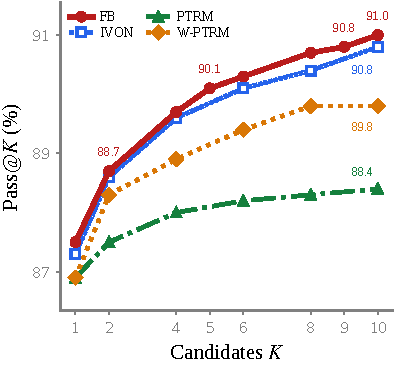
\includegraphics{figures/maze_hard_pass_at_k.pdf}
    \caption{Candidate coverage.}
    \label{fig:maze-hard-pass-at-k}
  \end{subfigure}\hfill
  \begin{subfigure}[t]{0.48\linewidth}
    \centering
    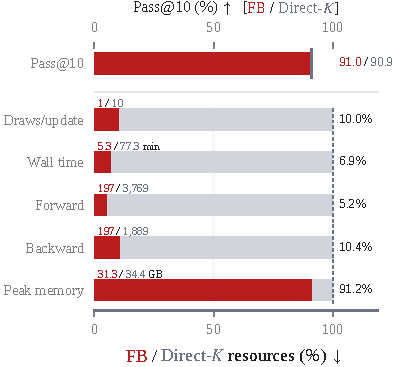
\includegraphics{figures/maze_hard_training_efficiency.pdf}
    \caption{Training resources.}
    \label{fig:maze-hard-training-efficiency}
  \end{subfigure}
  \caption{\textbf{FB improves inference and training efficiency on
  Maze-Hard.} (a) FB reaches each baseline's Pass@10 with fewer candidates
  using the same TRM backbone, 1,000 test problems, and reasoning depth 16.
  (b) At 188 updates, one-draw FB maintains comparable Pass@10 to
  Direct-$K{=}10$ while reducing training resources. Direct-$K$ uses seed 0;
  FB reports the mean over seeds 0--2.}
  \label{fig:maze-hard-efficiency}
\end{figure}

Using all saved FB prefixes to locate the first crossing, FB reaches PTRM's
Pass@10 of 88.4\% with two candidates, reducing solver executions by 80\%, and
reaches W-PTRM's 89.8\% with five candidates, reducing them by 50\%. FB also
reaches IVON's Pass@10 of 90.8\% with nine candidates, reducing solver
executions by 10\%; across the displayed budgets, FB exceeds IVON by
0.1--0.3 percentage points.

\subsection{Fidelity of one-draw finite-$K$ optimization}
\label{sec:objective-approximation}

We test whether one-draw FB follows the original finite-$K$ objective during
training.
\placeholder{Compare direct $K$-draw optimization, the naive one-sample
surrogate, and FB from matched initialization and training data. Add a
three-panel figure reporting (a) the true finite-$K$ objective estimated with
multiple posterior draws, (b) the saddle-objective gap, and (c) dual tracking
error over training.}

\subsection{Computational advantage of one-draw training}
\label{sec:computational-efficiency}

Direct finite-$K$ optimization requires $K$ solver executions per update,
whereas FB uses one.
At the matched endpoint of 188 updates,
\Cref{fig:maze-hard-training-efficiency} compares Direct-$K{=}10$ seed 0 with
the mean of FB seeds 0--2. FB attains 91.0\% Pass@10 versus 90.9\% for
Direct-$K$, while using 10.0\% as many posterior draws per update, 6.9\% of
the wall-clock time, 5.2\% of the forward passes, and 10.4\% of the backward
passes. Peak memory is reduced more modestly to 91.2\%. This endpoint
comparison supports comparable performance with substantially less training
compute; it does not establish a cost-to-target result.
